\scanpage{12}\mspage{9.}
\begingroup
\makeatletter\tagsleft@true\makeatother
From now on $\widetilde E$ has a cusp and $\widetilde E_0(k)=k^+$

\textcircled{3} Assume $\boxed{\mathfrak p\mid b_2}$. Then $\mathfrak p^2\nmid a_6\Longrightarrow\text{type }\mathrm{II}$, and
\[
 f=v(\Delta),\qquad c=1,\qquad \widetilde E_0(k)=k^+.
\]
[Proof. Consider the $2$-dimensional local ring $A=R[x,y]_m$, where $m=(\mathfrak p,x,y)$. It is regular because $a_6\in(x,y)\Rightarrow m=(x,y)$. Hence Weierstrass model $=$ Neron model]

\textcircled{4} Assume $\boxed{\mathfrak p^2\mid a_6}$ (which implies $\mathfrak p^2\mid b_6$ and $b_8$). Then $\mathfrak p^3\nmid b_8\Rightarrow\text{Type }\mathrm{III}$, and
\[
 f=v(\Delta)-1,\qquad c=2,\qquad \widetilde E_0(k)=k^+
\]
\reversemarginpar\margin{\deleted{\unsure{\textcircled{4}|\textcircled{5}}}}[Proof. let $\mathfrak p=\pi R$, and let $a_i=\pi^m a_{i,m}$, $x=\pi^m x_m$, $y=\pi^m y_m$, etc. Our equation can be written
\[
 y_1^2+a_{1,0}x_1y_1+a_{3,1}y_1=\pi x_1^3+a_{2,0}x_1^2+a_{4,1}x_1+a_{6,2}
 \tag*{(7.1)}
\]
The singular point on the fiber (whose local ring was $A$) blows up into the conic
\[
 Y^2+a_{1,0}XY+a_{3,1}Y\equiv a_{2,0}X^2+a_{4,1}X+a_{6,2},
 \tag*{($*$)}
\]
whose descriminant is $b_8\pi^{-2}=b_{8,2}$.]

\textcircled{5} Assume $\boxed{\mathfrak p^3\mid b_8}$ (which implies $\mathfrak p^2\mid b_4$). Then $\mathfrak p^3\nmid b_6\Rightarrow\text{type }\mathrm{IV}$, and
\[
\resizebox{\linewidth}{!}{$\displaystyle\begin{aligned}
 f&=v(\Delta)-2,\quad
 c=\left\{
 \begin{aligned}
 &3\ \text{if}\quad T^2+a_{3,1}T-a_{6,2}\equiv0\quad\text{has roots in }k.\\
 &1\ \text{if}\qquad\qquad\quad \text{''}\qquad\qquad\quad\text{has roots }\notin k
 \end{aligned}\right.,\quad \widetilde E_0(k)=k^+
\end{aligned}$}
\]

[Proof: The conic ($*$) becomes $T^2+a_{3,1}T-a_{6,2}=0$, where $T=Y-\alpha X$ is defined by $(Y-\alpha X)^2\equiv Y^2+a_1XY-a_2X^2$. The discriminant of $T^2+a_{3,1}T-a_{6,2}$ is $\pi^{-2} b_6=b_{6,2}$, so that if $\mathfrak p^3\nmid b_6$, then our conic degenerates into two \uline{distinct} lines. Dividing (7.1) by $x_1^3$, we get an equation of the form $F(U,V)=\pi$, where $F$ is a cubic with coeffs in $R$ which, mod $\pi$, factors into three distinct linear factors, $F\equiv L_1L_2L_3\pmod{\mathfrak p}$, such that the congruences $L_i\equiv0$ have a point in common. The local ring of that point is easily seen to be regular (the max ideal is generated by any two of the three factors $L_i$). Thus (7.1) gives a regular scheme over $R$ with fiber
\parbox[c]{1.48cm}{\setlength{\topsep}{0pt}\figure{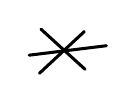
\begin{tikzpicture}[x=1cm,y=1cm,line width=1.1pt,line cap=round]
\draw (-.49,-.07) -- (.49,.05);
\draw (-.34,.26) -- (.22,-.25);
\draw (-.36,-.30) -- (.21,.23);
\end{tikzpicture}}}
consisting of three lines $L_i=0$, $i=1,2,3$ meeting in a point. Concerning the value of $c$, we see that $c$ is equal to the number of these lines which are rational over $k$. One of them is, and the others are given by $T^2+a_{3,1}T-a_{6,2}\equiv0$.
\normalmarginpar
\endgroup
% archive sheet number: 11
